\section{Лекция 4}

\subsection{\S XIII.3. Связь амплитуды рассеяния и сечения рассеяния}

\[
\psi^{(+)}(\vec{r})\big|_{r\to\infty} = e^{ikz} + f(\theta,\varphi)\,\frac{e^{ikr}}{r}
\qquad \vec{J}_i(\vec{r}) = A\,\vec{j}_i(\vec{r}), \quad \text{индекс } i \text{ --- падающий}
\]

\begin{figure}[H]
	\centering
	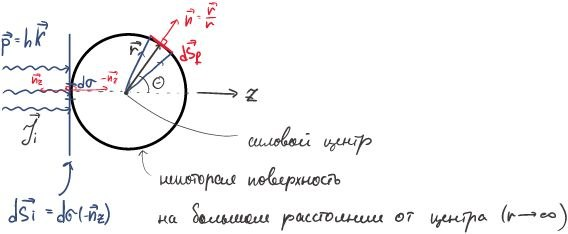
\includegraphics[width=0.8\linewidth]{images/l4_1.jpg}
\end{figure}

\[
\vec{j}(\vec{r}) = \frac{i \hbar}{2m}\bigl[(\nabla\psi^*)\psi - \psi^*(\nabla\psi)\bigr]
\]



Число частиц, падающих в единицу времени:
\[
\frac{dN_i}{dt} = \int \vec{J}_i(\vec{r})\,d\vec{S}_i = A\int \vec{j}_i(\vec{r})\,d\vec{S}_i = (*)
\]

Пусть соответствующая волновая функция $\Psi_E(\vec{r}) = \dfrac{1}{\sqrt{V}}\,e^{ikz} = \braket{\vec{r}}{\varphi^{(0)}}$ из уравнения Липпмана-Швингера.
Нормировка $V$ --- объем большой области.

\[
\Rightarrow j_i(\vec{r}) = \frac{1}{V}\,j(0, 0, v),\quad v = \frac{\hbar k}{m}
\]

\[
(*) = - \frac{A}{V}\,\frac{\hbar k}{m}\int d\sigma
\]

\[
\Rightarrow \frac{dN_i}{dt} = -\frac{A}{V}\,\frac{\hbar k}{m}\int d\sigma
\]

\[
\Rightarrow \frac{dN_f}{dt} = \int \vec{J}_f(\vec{r})\,d\vec{S}_f = A\int \vec{j}_f(\vec{r})\,d\vec{S}_f = (*)
\]

\[
d\vec{S}_f = r^2 d\Omega\,\vec{n}
\]

\[
(*) =  A\int j_f(\vec{r})\,\vec{n}\,r^2\,d\Omega = (*)
\]

Разложим $\vec{j}_f(\vec{r})$ в сферической системе скоординат: $\vec{j}_f(\vec{r}) = \vec{n}\,j_r(\vec{r}) + \vec{n}_\theta\,j_\theta + \vec{n}_\varphi\, j_f$

\[
\vec{\nabla} = \vec{n} \frac{\partial}{\partial \vec{r}} + \vec{n}_\theta\,\frac{\partial}{\partial\theta} + \vec{n}_\varphi\,\frac{1}{r\sin\theta}\frac{\partial}{\partial\varphi},
\quad \text{«выживает» только радиальная часть}
\]

\[
(*) =  A\int j_r(r)\,r^2\,d\Omega = (*)
\]

\[
j_r = \frac{1}{V}\,\frac{\hbar k}{m}\,\frac{1}{r^2}\,|f(\theta,\varphi)|^2
\]

\[
(*) = \frac{A\,\hbar k}{V\,m}\int_S d\Omega\,|f(\theta,\varphi)|^2
\]

Очевидно, что сколько частиц упало на поверхность, столько должно и покинуть ее, т.е. $\dfrac{dN_i}{dt} + \dfrac{dN_f}{dt} = 0$.

\[
\Rightarrow \frac{A}{V}\,\frac{\hbar k}{m}\int d\sigma = \frac{A\,\hbar k}{V\,m}\int d\Omega\,|f(\theta,\varphi)|^2
\qquad \Rightarrow \frac{d\sigma}{d\Omega} = |f(\theta,\varphi)|^2,
\]

где размерность $[d\sigma] = r^2 \Rightarrow$ это эффективная площадь. Здесь $d\sigma$ --- \textbf{дифференциальное сечение упругого рассеяния}. Тогда \textbf{полное сечение упругого рассеяния:}
\[
\sigma_{\text{tot}} = \int_\Omega d\Omega\left(\frac{d\sigma}{d\Omega}\right) = \int_\Omega |f(\theta,\varphi)|^2\,d\Omega
\]



\subsection{\S XIII.4. Оптическая теорема}

\begin{theorem}
	[оптическая] \emph{[Будет выведена на семинаре]}
	
	Полное сечение можно выразить через мнимую часть амплитуды рассеяния вперёд следующим образом:
	\[
	\sigma_{\text{tot}} = \frac{4\pi}{k}\int_0^{2\pi}\frac{d\varphi}{2\pi}\,\operatorname{Im}\bigl(f(\theta=0, \varphi)\bigr)
	\]
	
	Если потенциал центрально-симметричен:
	\[
	\sigma_{\text{tot}} = \frac{4\pi}{k}\,\operatorname{Im}\,f(\theta=0)
	\]
\end{theorem}


\subsection{\S XIII.5. Борновские приближения}

Решение возмущённой задачи в $1^\text{ом}$ борновском приближении: $\ket{\psi^{(+)}} = (\hat{1} + \hat{G}_0^{(+)}\hat{V})\ket{\varphi^{(0)}}$.

В координатном представлении с нормировкой на объем:
\[
\frac{\psi^{(+)}(\vec{r})}{\sqrt{V}} = \Psi_E(\vec{r}) + \frac{1}{\sqrt{V}}\,f^{(1)}(\theta,\varphi)\,\frac{e^{ikr}}{2}
\]

В первом борновском приближении:
\begin{align*}
	f^{(1)}(\theta,\varphi)
	&= -\frac{m \sqrt{V}}{2\pi\hbar^2} \int d\vec{r'}\,C^{-i(\vec{k'}\vec{r'})}\,V(\vec{r'})\,\psi_{(+)}(\vec{r'})
	= -\frac{m\sqrt{V}}{2\pi\hbar^2} \int d\vec{r'}\,C^{-i(\vec{k'}\vec{r'})}\,V(\vec{r'})\,\Psi_E(\vec{r'}) =\\
	&= -\frac{m}{2\pi\hbar^2} \int d\vec{r'}\,e^{-i\vec{r'}(\vec{k'} - \vec{k})}V(\vec{r'})
\end{align*}
Заметим, что получившийся интеграл является Фурье-преобразованием $V$ в координатном представлении.\\

В центрально-симметричном потенциале обозначим $\vec{q} = \vec{k'} - \vec{k}$, $q = |\vec{q}|$. Тогда $f^{(1)}(\theta) = -\dfrac{2m}{\hbar q}\int_0^\infty dr'\,r'\,V(r')\sin(q r')$. Где $\theta$?

\[
|\vec{k}| = |\vec{k'}| = k \Rightarrow q = 2k\sin\frac{\theta}{2}
\]

Пусть $ \Psi_E(\vec{r}) = \frac{e^{ikz}}{\sqrt{V}},\qquad \Psi_r(\vec{r}) = \frac{f(\theta,\varphi)}{\sqrt{V}}\,\frac{e^{ikr}}{2}$

Борновское приближение \underline{применимо}, когда $\|\Psi_E\|^2 \gg \|\Psi_r\|^2$, $\|\Psi_E\| = \tfrac{1}{\sqrt{V}}$ $\Rightarrow$

\[
\|\sqrt{V}\,\Psi_r\| \ll 1
\]

Другие способов записать условие применимости:
\begin{enumerate}
	\item $a$ --- радиус действия потенциала $\Rightarrow$ медленные частицы, т.е. $ka \ll 1$.
	
	$V_0$ --- хар. значение потенциала $\Rightarrow$ условие = $|V_0| \ll \dfrac{\hbar^2}{m a^2}$ (малая сила).
	
	\item Быстрые частицы, т.е. $ka \gg 1$
	
	$\Rightarrow$ условие = $|V_0| \ll \dfrac{\hbar^2}{ma}\,ka)$.
\end{enumerate}

Т.е. приближение 1) работает и для медленных, и для быстрых частиц.




\section{X. Запутанные состояния и неравенства Белла}

\subsection{\S X.1. Матрица плотности подсистемы}

Пусть некоторая система состоит из двух подсистем, каждая из которых живёт в своём подпространстве: $\mathcal{H}^{(1)}$ и $\mathcal{H}^{(2)}$. Вся система в $\mathcal{H} = \mathcal{H}^{(1)} \otimes \mathcal{H}^{(2)}$. известна матрица плотности полной системы $\hat{\rho}$. Хотим найти матрицы подсистем $\hat{\rho}^{(1)}$ и $\hat{\rho}^{(2)}$.\\

Пусть имеется какая-то наблюдаемая $F^{(1)}$ только в $\mathcal{H}^{(1)}$ $\Rightarrow$
$\hat{\mathcal{F}}^{(1)} = \hat{F}^{(1)} \otimes \hat{1}^{(2)}$ (дополнено до действия в $\mathcal{H}$).\\

Введём в $\mathcal{H}^{(1)}$ ортонормированный базис $\{|a_j^{(1)}\rangle\}$, $\braket{a_j^{(1)}}{a_{i}^{(1)}} = \delta_{ij}$ $\Rightarrow$

\begin{align*}
	\langle F^{(1)}\rangle
	&= \langle F^{(1)}\rangle_{\rho^{(1)}} = \mathrm{Tr}\,(\hat{F}^{(1)}\hat{\rho}^{(1)})
	= \sum_j \braupket{a_j^{(1)}}{\hat{F}^{(1)}\hat{\rho}^{(1)}}{a_j^{(1)}} = \\
	&= \sum\limits_{jj'}\braupket{a_j^{(1)}}{\hat{F}^{(1)}}{a_{j'}^{(1)}}\braupket{a_{j'}^{(1)}}{\hat{\rho}^{(1)}}{a_{j}^{(1)}}
\end{align*}

В $\mathcal{H}^{(2)}$ введем ортонормированный базис $\{|b_l^{(2)}\rangle\}$, $\braket{b_l^{(2)}}{b_{l'}^{(2)}} = \delta_{ll'}$ $\Rightarrow$ в $\mathcal{H}$ можно ввести естественный базис $\ket{\eta_{\alpha=\{j, l\}}} = \ket{a_j^{(1)}}\otimes\ket{b_l^{(2)}}$. Тогда

\[
	\langle F^{(1)}\rangle = \langle \mathcal{F}^{(1)} \rangle_{\rho} = \mathrm{Tr}_{\mathcal{H}}(\hat{\mathcal{F}}^{(1)}\hat{\rho}) =
\]
\[
 =  \sum_\alpha \braupket{\eta_\alpha}{\hat{\mathcal{F}}^{(1)}\hat{\rho}}{\eta_\alpha} = \sum\limits_{j, l}\sum\limits_{j', l' }\braupket{a_j^{(1)}}{\hat{F}^{(1)}}{a_{j'}^{(1)}}\braupket{b_{l}^{(2)}}{\hat{1}^{(2)}}{b_{l'}^{(2)}}\braupket{\eta_{\alpha'}}{\hat{\rho}}{\eta_\alpha} = 
\]
\[
= \sum\limits_{j, l, j'}\braupket{a_j^{(1)}}{\hat{F}^{(1)}}{a_{j'}^{(1)}} \bra{a_{j'}^{(1)}}\braupket{b_l^{(2)}}{\hat{\rho}}{b_{l'}^{(2)}}\ket{a_j^{(1)}} = \sum\limits_{j, j'}\braupket{a_j^{(1)}}{\hat{F}^{(1)}}{a_{j'}^{(1)}} \bra{a_{j'}^{(1)}}\Big(\sum_l\braupket{b_l^{(2)}}{\hat{\rho}}{b_{l'}^{(2)}}\Big)\ket{a_j^{(1)}}
\]

Тогда, приравнивая $\langle F^{(1)}\rangle$ через $\rho^{(1)}$ и $\rho$, получим
\[
\hat{\rho}^{(1)} = \sum_l \braupket{b_l^{(2)}}{\hat{\rho}}{b_{l'}^{(2)}} := \mathrm{Tr}_{\mathcal{H}^{(2)}}\hat{\rho}
\]
--- \textbf{частичный след} в гильбертовом пространстве $\mathcal{H}^{(2)}$.\\


Аналогично $\hat{\rho}^{(2)} = \mathrm{Tr}_{\mathcal{H}^{(1)}}\hat{\rho}$.

\subsection{\S X.2. Запутанные, факторизованные и сепарабельные состояния}

Рассмотрим квантовую систему из $N$ подсистем.\\

Обозначим чистые состояния как $\ket{\Psi} \in \mathcal{H} = \mathcal{H}^{(1)} \otimes \cdots \otimes \mathcal{H}^{(N)}$.\\

В $\mathcal{H}$ можно ввести естественный базис: $\ket{\eta_\alpha} = \ket{a_j^{(1)}}\otimes\ket{b_\ell^{(2)}} \otimes \cdots \otimes |c_k^{(N)}\rangle$ $\Rightarrow$ 

\[
\ket{\Psi} = \displaystyle\sum_{\alpha=\{j,\ell,\ldots,k\}} C_\alpha\ket{\eta_\alpha}
\]

\begin{definition}
	Предположим, что мы построили все возможные базисы из прямых произведений всех возможных базисов $\mathcal{H}^{(1)} \ldots\mathcal{H}^{(N)}$ из $\mathcal{H}$ и все возможные разложения $\ket{\Psi}$.
	Если при всех этих разложениях в $\displaystyle\sum_\alpha C_\alpha\ket{\eta_\alpha}$ всегда $\geq 2$ $C_\alpha \neq 0$, то такое состояние называется \textbf{запутанным}.\\
	
	Если при переборе всех базисов нашли такой, что $\ket{\Psi} = \ket{\varphi_{j^{(1)}}^{(1)}} \otimes \ket{\chi_{l^{(2)}}^{(2)}} \otimes \cdots \otimes \ket{\kappa_{k^{(N)}}^{(N)}}$, тогда такое состояние называется \textbf{факторизованным}.
\end{definition}


$\Rightarrow$ все состояния делятся на два этих класса.
